\chapter{Constellation Diagrams}
\label{ch:constellation-diagrams}

\begin{nontechnical}
\textbf{A constellation diagram is like a visual map showing all possible ``hand signals'' your phone can use to send data}---each dot represents a unique signal position!

\textbf{The lighthouse analogy:}
\begin{itemize}
\item Imagine communicating with lighthouse beams
\item You can vary \textbf{brightness} (amplitude) and \textbf{color} (phase)
\item Each unique combination = one symbol (represents bits)
\item Constellation diagram = map of all possible combinations
\end{itemize}

\textbf{Real example:} WiFi uses 64-QAM (64 dots = 6 bits per symbol) in good conditions, drops to QPSK (4 dots = 2 bits per symbol) when signal is weak.

\textbf{Why it matters:} More dots = faster data, but dots must be well-separated to distinguish in noise. Your phone constantly monitors dot scatter and adapts the constellation for optimal speed vs. reliability!
\end{nontechnical}

\section{Overview}

A \textbf{constellation diagram} is a two-dimensional graphical representation of digital modulation schemes in the complex I/Q plane. Each point represents a unique symbol that encodes binary data through specific amplitude and phase combinations of the carrier signal.

\begin{keyconcept}
The constellation diagram is the \textbf{most intuitive visualization} of digital communication quality. Tight symbol clusters indicate excellent signal-to-noise ratio, while scattered clouds reveal channel degradation requiring error correction or reduced data rate.
\end{keyconcept}

Constellation diagrams serve three critical purposes in modern communications:
\begin{enumerate}
\item \textbf{Modulation design:} Optimizing symbol placement for maximum noise immunity
\item \textbf{Real-time diagnostics:} Identifying channel impairments and synchronization errors
\item \textbf{Adaptive systems:} Enabling automatic modulation selection based on link quality
\end{enumerate}

\section{Mathematical Description}

\subsection{Complex Baseband Representation}

Every modulated symbol can be represented as a complex number in baseband:
\begin{equation}
s_k = I_k + jQ_k = A_k e^{j\phi_k}
\end{equation}
where:
\begin{itemize}
\item $s_k$ = complex symbol for the $k$-th transmission interval
\item $I_k$ = in-phase component (real axis projection)
\item $Q_k$ = quadrature component (imaginary axis projection)
\item $A_k = \sqrt{I_k^2 + Q_k^2}$ = symbol amplitude
\item $\phi_k = \arctan(Q_k/I_k)$ = symbol phase (radians)
\end{itemize}

\subsection{Passband Signal Mapping}

The complex baseband symbol maps to a real-valued passband waveform:
\begin{equation}
x(t) = \mathrm{Re}\{s_k \cdot e^{j2\pi f_c t}\} = I_k\cos(2\pi f_c t) - Q_k\sin(2\pi f_c t)
\end{equation}
where:
\begin{itemize}
\item $f_c$ = carrier frequency (Hz)
\item $t \in [kT_s, (k+1)T_s]$ = time interval for symbol $k$
\item $T_s$ = symbol period (seconds)
\end{itemize}

This representation shows how I/Q coordinates directly control the carrier's amplitude and phase.

\subsection{Symbol Set Definition}

For an $M$-ary modulation scheme, the constellation consists of $M$ complex symbols:
\begin{equation}
\mathcal{S} = \{s_0, s_1, s_2, \ldots, s_{M-1}\}
\end{equation}
where each symbol $s_m$ represents $\log_2(M)$ bits of information.

\textbf{Examples:}
\begin{itemize}
\item BPSK: $M = 2$, 1 bit/symbol, $\mathcal{S} = \{+A, -A\}$
\item QPSK: $M = 4$, 2 bits/symbol, $\mathcal{S} = \{A/\sqrt{2}(1 \pm j), A/\sqrt{2}(-1 \pm j)\}$
\item 16-QAM: $M = 16$, 4 bits/symbol, rectangular grid of 16 points
\item 64-QAM: $M = 64$, 6 bits/symbol, rectangular grid of 64 points
\end{itemize}

\section{Standard Constellation Types}

\subsection{Phase Shift Keying (PSK) Constellations}

PSK constellations place all symbols on a circle of constant radius $A$, varying only phase.

\subsubsection{Binary PSK (BPSK)}

\begin{center}
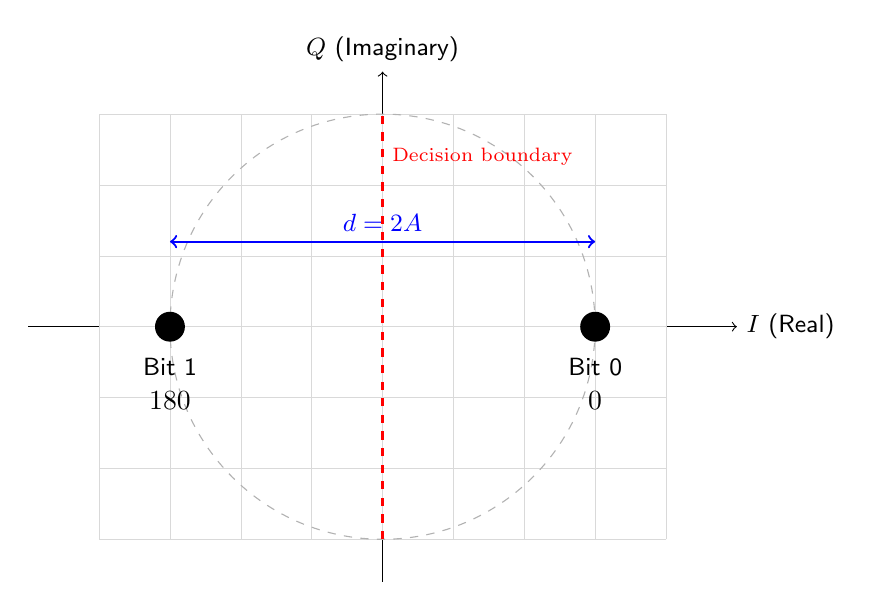
\begin{tikzpicture}[scale=1.8]
% Axes
\draw[->] (-2.5,0) -- (2.5,0) node[right] {\sffamily\small $I$ (Real)};
\draw[->] (0,-1.8) -- (0,1.8) node[above] {\sffamily\small $Q$ (Imaginary)};

% Grid
\draw[very thin,gray!30] (-2,-1.5) grid[step=0.5] (2,1.5);

% Circle showing constant amplitude
\draw[dashed,gray!60] (0,0) circle (1.5);

% Constellation points
\fill[black] (-1.5,0) circle (3pt);
\fill[black] (1.5,0) circle (3pt);

% Labels
\node[below=8pt,align=center] at (-1.5,0) {\sffamily\small Bit 1\\$180°$};
\node[below=8pt,align=center] at (1.5,0) {\sffamily\small Bit 0\\$0°$};

% Distance annotation
\draw[<->,thick,blue] (-1.5,0.6) -- (1.5,0.6) node[midway,above] {\sffamily\small $d = 2A$};

% Decision boundary
\draw[red,thick,dashed] (0,-1.5) -- (0,1.5);
\node[red,right,font=\scriptsize] at (0,1.2) {Decision boundary};
\end{tikzpicture}
\end{center}

\textbf{Properties:}
\begin{itemize}
\item 2 symbols, 1 bit/symbol
\item Maximum Euclidean distance for binary modulation
\item Immune to amplitude variations (constant envelope)
\item Requires carrier phase synchronization
\end{itemize}

\subsubsection{Quadrature PSK (QPSK)}

\begin{center}
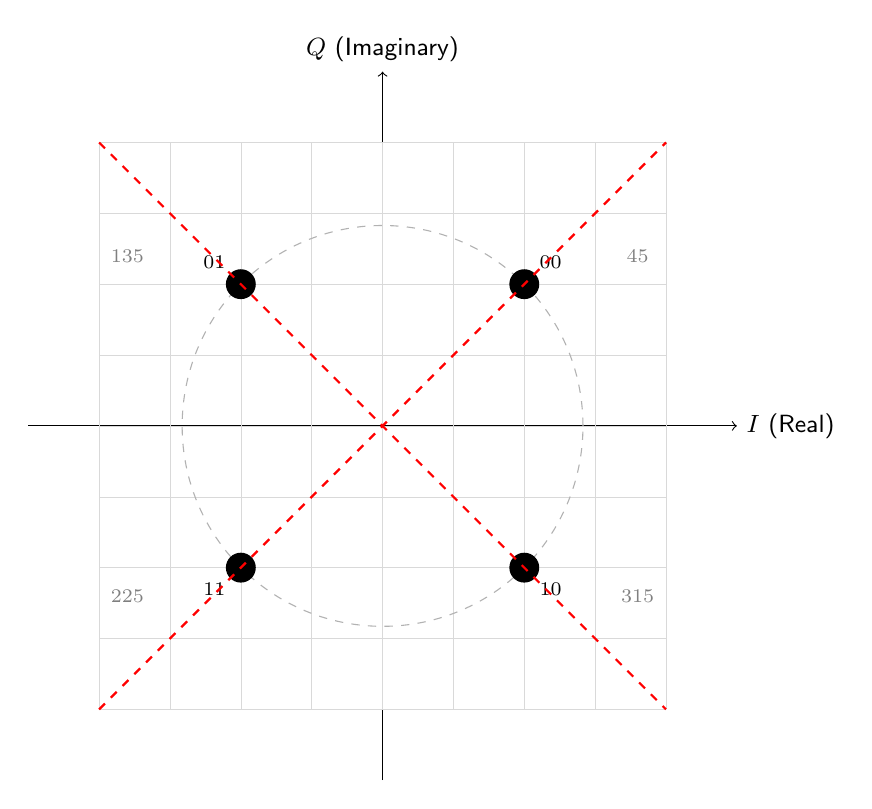
\begin{tikzpicture}[scale=1.8]
% Axes
\draw[->] (-2.5,0) -- (2.5,0) node[right] {\sffamily\small $I$ (Real)};
\draw[->] (0,-2.5) -- (0,2.5) node[above] {\sffamily\small $Q$ (Imaginary)};

% Grid
\draw[very thin,gray!30] (-2,-2) grid[step=0.5] (2,2);

% Circle showing constant amplitude
\draw[dashed,gray!60] (0,0) circle (1.414);

% Constellation points (at 45°, 135°, 225°, 315°)
\fill[black] (1,1) circle (3pt);
\fill[black] (-1,1) circle (3pt);
\fill[black] (-1,-1) circle (3pt);
\fill[black] (1,-1) circle (3pt);

% Labels with bit mappings (Gray coding)
\node[above right=2pt,font=\scriptsize] at (1,1) {00};
\node[above left=2pt,font=\scriptsize] at (-1,1) {01};
\node[below left=2pt,font=\scriptsize] at (-1,-1) {11};
\node[below right=2pt,font=\scriptsize] at (1,-1) {10};

% Phase angles
\node[font=\scriptsize,gray] at (1.8,1.2) {$45°$};
\node[font=\scriptsize,gray] at (-1.8,1.2) {$135°$};
\node[font=\scriptsize,gray] at (-1.8,-1.2) {$225°$};
\node[font=\scriptsize,gray] at (1.8,-1.2) {$315°$};

% Decision boundaries
\draw[red,thick,dashed] (-2,-2) -- (2,2);
\draw[red,thick,dashed] (-2,2) -- (2,-2);
\end{tikzpicture}
\end{center}

\textbf{Properties:}
\begin{itemize}
\item 4 symbols, 2 bits/symbol
\item Symbols at $45°$, $135°$, $225°$, $315°$ (Gray coded)
\item Constant envelope (compatible with nonlinear amplifiers)
\item Minimum symbol distance: $d_{\min} = A\sqrt{2}$
\end{itemize}

\subsection{Quadrature Amplitude Modulation (QAM)}

QAM constellations use both amplitude and phase variations, arranged in rectangular grids.

\subsubsection{16-QAM Constellation}

\begin{center}
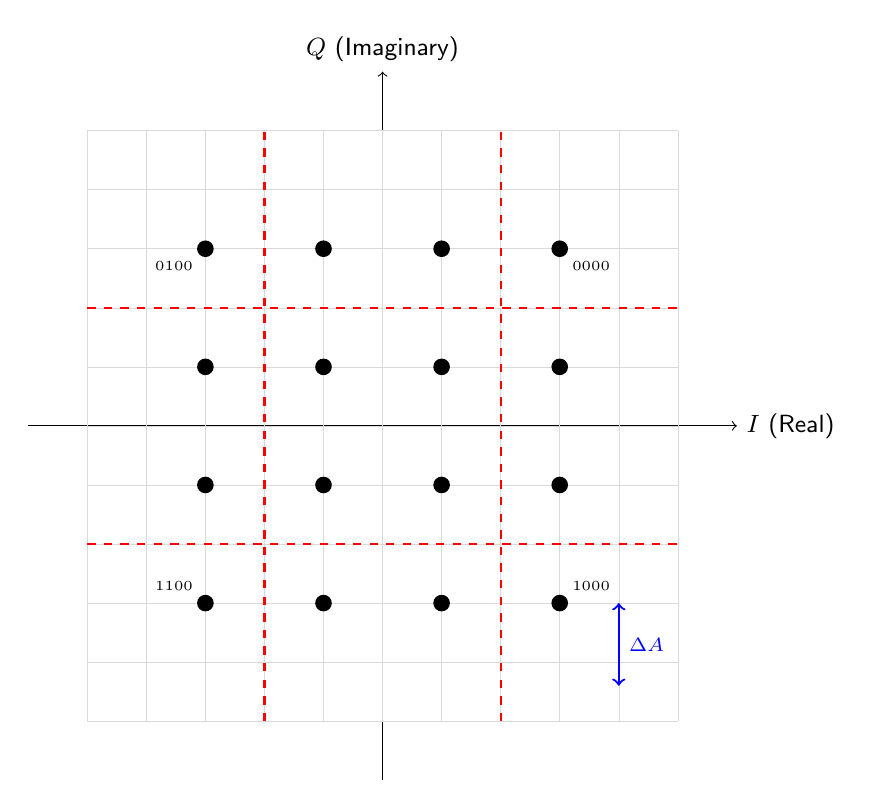
\begin{tikzpicture}[scale=1.5]
% Axes
\draw[->] (-3,0) -- (3,0) node[right] {\sffamily\small $I$ (Real)};
\draw[->] (0,-3) -- (0,3) node[above] {\sffamily\small $Q$ (Imaginary)};

% Grid
\draw[very thin,gray!30] (-2.5,-2.5) grid[step=0.5] (2.5,2.5);

% 16-QAM constellation points (4×4 grid)
\foreach \i in {-1.5,-0.5,0.5,1.5} {
  \foreach \q in {-1.5,-0.5,0.5,1.5} {
    \fill[black] (\i,\q) circle (2pt);
  }
}

% Sample bit labels on corner points
\node[below right=1pt,font=\tiny] at (1.5,1.5) {0000};
\node[below left=1pt,font=\tiny] at (-1.5,1.5) {0100};
\node[above left=1pt,font=\tiny] at (-1.5,-1.5) {1100};
\node[above right=1pt,font=\tiny] at (1.5,-1.5) {1000};

% Decision boundaries (sample)
\draw[red,thick,dashed] (-1,-2.5) -- (-1,2.5);
\draw[red,thick,dashed] (1,-2.5) -- (1,2.5);
\draw[red,thick,dashed] (-2.5,-1) -- (2.5,-1);
\draw[red,thick,dashed] (-2.5,1) -- (2.5,1);

% Amplitude levels annotation
\draw[<->,blue,thick] (2,-2.2) -- (2,-1.5) node[midway,right,font=\scriptsize] {$\Delta A$};
\end{tikzpicture}
\end{center}

\textbf{Properties:}
\begin{itemize}
\item 16 symbols, 4 bits/symbol
\item Non-constant envelope (requires linear amplifiers)
\item Higher spectral efficiency than QPSK
\item Minimum symbol distance: $d_{\min} = 2\Delta A$ where $\Delta A$ is grid spacing
\end{itemize}

\section{Decision Regions and Symbol Detection}

\subsection{Maximum Likelihood Detection}

The receiver decides which symbol $\hat{s}_k$ was transmitted by finding the closest constellation point to the received signal $r_k$:
\begin{equation}
\hat{s}_k = \arg\min_{s_m \in \mathcal{S}} |r_k - s_m|^2
\end{equation}
where:
\begin{itemize}
\item $r_k = s_k + n_k$ = received signal (symbol + noise)
\item $n_k$ = complex AWGN with variance $\sigma^2$ per dimension
\item $|r_k - s_m|$ = Euclidean distance in I/Q plane
\end{itemize}

This is equivalent to choosing the symbol in whose Voronoi region $r_k$ falls.

\subsection{Decision Boundaries}

Decision boundaries are perpendicular bisectors between adjacent constellation points. For rectangular QAM:
\begin{equation}
\text{I-axis boundaries: } I = \pm \Delta A, \pm 3\Delta A, \ldots
\end{equation}
\begin{equation}
\text{Q-axis boundaries: } Q = \pm \Delta A, \pm 3\Delta A, \ldots
\end{equation}
where $\Delta A$ is the spacing between adjacent amplitude levels.

\begin{calloutbox}{Gray Coding for Error Minimization}
Constellation points are typically labeled using \textbf{Gray coding}, where adjacent symbols differ by only one bit. This ensures that symbol errors (most likely between neighbors) cause only single-bit errors, reducing the bit error rate.

\textbf{Example (QPSK):} 00 $\rightarrow$ 01 $\rightarrow$ 11 $\rightarrow$ 10 (circular sequence with 1-bit changes)
\end{calloutbox}

\subsection{Symbol Error Probability}

For M-QAM in AWGN with average symbol energy $E_s$ and noise spectral density $N_0$:
\begin{equation}
P_s \approx 4\left(1 - \frac{1}{\sqrt{M}}\right) Q\left(\sqrt{\frac{3E_s}{(M-1)N_0}}\right)
\end{equation}
where:
\begin{itemize}
\item $P_s$ = symbol error probability
\item $M$ = constellation size
\item $Q(x) = \frac{1}{\sqrt{2\pi}}\int_x^\infty e^{-t^2/2}\,dt$ = Gaussian Q-function
\item $E_s = \frac{1}{M}\sum_{m=0}^{M-1}|s_m|^2$ = average symbol energy
\end{itemize}

For QPSK specifically (equivalent to two independent BPSK channels):
\begin{equation}
P_s = 2Q\left(\sqrt{\frac{2E_s}{N_0}}\right) - Q^2\left(\sqrt{\frac{2E_s}{N_0}}\right) \approx 2Q\left(\sqrt{\frac{2E_s}{N_0}}\right)
\end{equation}

\section{Channel Impairments on Constellations}

\subsection{Additive White Gaussian Noise (AWGN)}

Noise adds a random complex value $n_k = n_I + jn_Q$ to each symbol, where $n_I$ and $n_Q$ are independent Gaussian random variables with variance $\sigma^2 = N_0/2$ per dimension.

\textbf{Effect:} Received symbols form Gaussian clouds around ideal positions.

\begin{center}
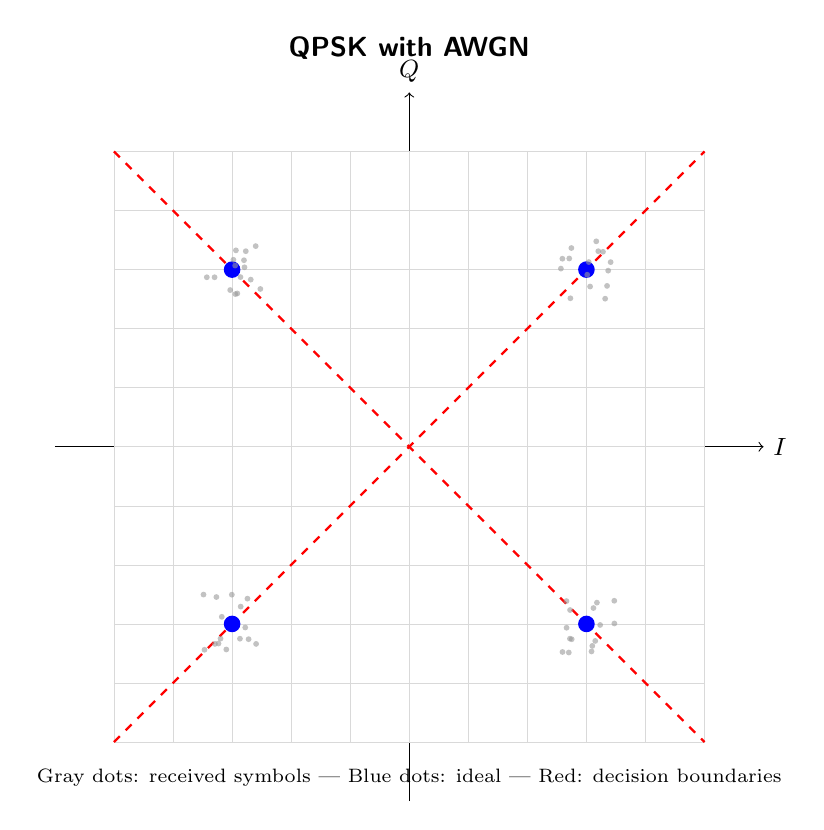
\begin{tikzpicture}[scale=1.5]
% Title
\node[above,font=\sffamily\bfseries] at (0,3.2) {QPSK with AWGN};

% Axes
\draw[->] (-3,0) -- (3,0) node[right] {\sffamily\small $I$};
\draw[->] (0,-3) -- (0,3) node[above] {\sffamily\small $Q$};

% Grid
\draw[very thin,gray!30] (-2.5,-2.5) grid[step=0.5] (2.5,2.5);

% Decision boundaries
\draw[red,thick,dashed] (-2.5,-2.5) -- (2.5,2.5);
\draw[red,thick,dashed] (-2.5,2.5) -- (2.5,-2.5);

% Ideal constellation points
\fill[blue] (1.5,1.5) circle (2pt);
\fill[blue] (-1.5,1.5) circle (2pt);
\fill[blue] (-1.5,-1.5) circle (2pt);
\fill[blue] (1.5,-1.5) circle (2pt);

% Noise clouds (scattered points around each symbol)
\foreach \i in {1,...,15} {
  \pgfmathsetmacro{\randI}{1.5 + 0.25*rand}
  \pgfmathsetmacro{\randQ}{1.5 + 0.25*rand}
  \fill[black!40,opacity=0.6] (\randI,\randQ) circle (0.7pt);
}
\foreach \i in {1,...,15} {
  \pgfmathsetmacro{\randI}{-1.5 + 0.25*rand}
  \pgfmathsetmacro{\randQ}{1.5 + 0.25*rand}
  \fill[black!40,opacity=0.6] (\randI,\randQ) circle (0.7pt);
}
\foreach \i in {1,...,15} {
  \pgfmathsetmacro{\randI}{-1.5 + 0.25*rand}
  \pgfmathsetmacro{\randQ}{-1.5 + 0.25*rand}
  \fill[black!40,opacity=0.6] (\randI,\randQ) circle (0.7pt);
}
\foreach \i in {1,...,15} {
  \pgfmathsetmacro{\randI}{1.5 + 0.25*rand}
  \pgfmathsetmacro{\randQ}{-1.5 + 0.25*rand}
  \fill[black!40,opacity=0.6] (\randI,\randQ) circle (0.7pt);
}

% Legend
\node[font=\scriptsize] at (0,-2.8) {Gray dots: received symbols | Blue dots: ideal | Red: decision boundaries};
\end{tikzpicture}
\end{center}

\subsection{Phase Noise and Carrier Offset}

A phase error $\phi_e$ rotates the entire constellation:
\begin{equation}
r_k = s_k \cdot e^{j\phi_e} + n_k
\end{equation}

\textbf{Effect:} Constellation rotates by angle $\phi_e$. Small offsets cause symbol errors; large offsets require carrier recovery.

\subsection{Amplitude Imbalance and Distortion}

Non-uniform amplifier gain compresses outer symbols:
\begin{equation}
r_k = f(|s_k|) \cdot e^{j\angle s_k} + n_k
\end{equation}
where $f(|s_k|)$ is a nonlinear amplitude response.

\textbf{Effect:} QAM constellations show compressed outer rings. Requires predistortion or backoff.

\section{Error Vector Magnitude (EVM)}

\subsection{Definition}

EVM quantifies constellation quality as the RMS error between received and ideal symbols:
\begin{equation}
\mathrm{EVM} = \sqrt{\frac{1}{N}\sum_{k=1}^{N}\frac{|r_k - s_k|^2}{|s_k|^2}} \times 100\%
\end{equation}
where:
\begin{itemize}
\item $N$ = number of measured symbols
\item $r_k$ = received symbol
\item $s_k$ = nearest ideal constellation point
\end{itemize}

\subsection{Relationship to SNR}

For small EVM, the relationship to SNR is approximately:
\begin{equation}
\mathrm{SNR}_{\text{dB}} \approx -20\log_{10}\left(\frac{\mathrm{EVM}}{100\%}\right)
\end{equation}

\textbf{Practical benchmarks:}

\begin{center}
\begin{tabular}{@{}lrll@{}}
\toprule
Modulation & EVM Limit & SNR Requirement & Application \\
\midrule
QPSK & 17.5\% & 15~dB & Cellular control channels \\
16-QAM & 12.5\% & 18~dB & WiFi 802.11n \\
64-QAM & 8.0\% & 22~dB & LTE/5G high throughput \\
256-QAM & 3.5\% & 29~dB & Cable modem DOCSIS 3.1 \\
1024-QAM & 2.0\% & 34~dB & WiFi 6E (802.11ax) \\
\bottomrule
\end{tabular}
\end{center}

\begin{warningbox}
\textbf{EVM must be measured under realistic conditions.} Lab equipment may show excellent EVM, but real-world performance depends on amplifier linearity, phase noise, I/Q imbalance, and multipath interference. Always verify EVM at the antenna output, not the baseband DAC.
\end{warningbox}

\section{Practical Applications}

\subsection{Adaptive Modulation in LTE/5G}

Cellular base stations continuously measure downlink channel quality and select the highest viable modulation:

\begin{center}
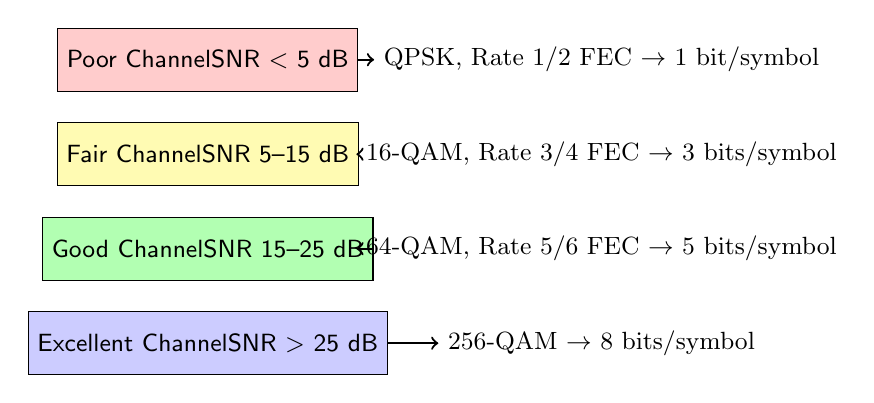
\begin{tikzpicture}[
  block/.style={rectangle, draw, minimum width=3cm, minimum height=0.8cm, font=\sffamily\small},
  node distance=1.2cm
]
% Channel quality blocks
\node[block,fill=red!20] (poor) {Poor Channel\\SNR $<$ 5 dB};
\node[block,fill=yellow!30,below of=poor] (fair) {Fair Channel\\SNR 5--15 dB};
\node[block,fill=green!30,below of=fair] (good) {Good Channel\\SNR 15--25 dB};
\node[block,fill=blue!20,below of=good] (excellent) {Excellent Channel\\SNR $>$ 25 dB};

% Modulation choices
\node[right of=poor,node distance=5cm,font=\small] (mod1) {QPSK, Rate 1/2 FEC $\rightarrow$ 1 bit/symbol};
\node[right of=fair,node distance=5cm,font=\small] (mod2) {16-QAM, Rate 3/4 FEC $\rightarrow$ 3 bits/symbol};
\node[right of=good,node distance=5cm,font=\small] (mod3) {64-QAM, Rate 5/6 FEC $\rightarrow$ 5 bits/symbol};
\node[right of=excellent,node distance=5cm,font=\small] (mod4) {256-QAM $\rightarrow$ 8 bits/symbol};

% Arrows
\draw[->,thick] (poor) -- (mod1);
\draw[->,thick] (fair) -- (mod2);
\draw[->,thick] (good) -- (mod3);
\draw[->,thick] (excellent) -- (mod4);
\end{tikzpicture}
\end{center}

This \textbf{link adaptation} maximizes throughput while maintaining target error rates (typically $10^{-3}$ to $10^{-6}$ post-FEC).

\subsection{Cable Modem DOCSIS 3.1}

DOCSIS 3.1 uses constellations up to \textbf{4096-QAM} (12 bits/symbol) for downstream channels with excellent SNR:

\begin{itemize}
\item \textbf{Modulation profile:} Adaptive per subcarrier based on channel response
\item \textbf{Frequency range:} 88--1218~MHz (1.2~GHz bandwidth)
\item \textbf{Subcarrier spacing:} 25--50~kHz (OFDM with 4096 subcarriers)
\item \textbf{Peak throughput:} 10~Gbps downstream (with bonding)
\end{itemize}

\subsection{WiFi 6E (802.11ax) Constellation Shaping}

WiFi 6E supports 1024-QAM but uses \textbf{probabilistic constellation shaping} (PCS) to:
\begin{enumerate}
\item Reduce transmit power by favoring low-amplitude symbols
\item Maintain spectral efficiency near Shannon capacity
\item Improve battery life on mobile devices
\end{enumerate}

\section{Worked Example: 16-QAM Link Budget}

\textbf{Scenario:} Design a 16-QAM wireless link for 10~Mbps data rate

\subsection*{Given Parameters}

\begin{tabular}{@{}ll@{}}
Modulation & 16-QAM (4 bits/symbol) \\
Symbol rate & $R_s = 10 \times 10^6 / 4 = 2.5$~Msymbols/s \\
Bandwidth (RRC, $\alpha=0.25$) & $B = 2.5 \times 1.25 = 3.125$~MHz \\
Required $E_s/N_0$ for BER $10^{-6}$ & 18.5~dB \\
TX power & $P_t = 30$~dBm (1~W) \\
TX antenna gain & $G_t = 10$~dBi \\
Distance & $d = 1$~km \\
Frequency & $f = 2.4$~GHz \\
RX antenna gain & $G_r = 10$~dBi \\
RX noise figure & $NF = 5$~dB \\
\end{tabular}

\subsection*{Step 1: Free-Space Path Loss}

\begin{equation}
\mathrm{FSPL} = 20\log_{10}(d_{\text{km}}) + 20\log_{10}(f_{\text{MHz}}) + 32.45
\end{equation}
\begin{equation}
\mathrm{FSPL} = 20\log_{10}(1) + 20\log_{10}(2400) + 32.45 = 100.0~\text{dB}
\end{equation}

\subsection*{Step 2: Received Signal Power}

\begin{equation}
P_r = P_t + G_t + G_r - \mathrm{FSPL} = 30 + 10 + 10 - 100 = -50~\text{dBm}
\end{equation}

\subsection*{Step 3: Noise Power}

System noise temperature: $T_s = T_0 \cdot 10^{NF/10} = 290 \times 10^{0.5} = 916$~K

\begin{equation}
N = kT_sB = (1.38 \times 10^{-23})(916)(3.125 \times 10^6) = 3.95 \times 10^{-14}~\text{W}
\end{equation}
\begin{equation}
N_{\text{dBm}} = 10\log_{10}(3.95 \times 10^{-14} / 10^{-3}) = -104.0~\text{dBm}
\end{equation}

\subsection*{Step 4: Carrier-to-Noise Ratio}

\begin{equation}
\mathrm{CNR} = P_r - N = -50 - (-104) = 54.0~\text{dB}
\end{equation}

\subsection*{Step 5: Symbol Energy to Noise Ratio}

\begin{equation}
\frac{E_s}{N_0} = \mathrm{CNR} - 10\log_{10}(R_s) + 10\log_{10}(B)
\end{equation}
\begin{equation}
\frac{E_s}{N_0} = 54.0 - 10\log_{10}(2.5 \times 10^6) + 10\log_{10}(3.125 \times 10^6) = 54.0 - 64.0 + 65.0 = 55.0~\text{dB}
\end{equation}

Wait, let me recalculate more carefully:
\begin{equation}
\frac{E_s}{N_0} = \frac{P_r/R_s}{N_0} = \frac{P_r}{R_s} \cdot \frac{1}{N_0}
\end{equation}

Converting to dB:
\begin{equation}
\left(\frac{E_s}{N_0}\right)_{\text{dB}} = P_r(\text{dBm}) - N_0(\text{dBm/Hz}) - 10\log_{10}(R_s)
\end{equation}

where $N_0 = kT_s = (1.38 \times 10^{-23})(916) = 1.26 \times 10^{-20}$~W/Hz $= -169$~dBm/Hz

\begin{equation}
\left(\frac{E_s}{N_0}\right)_{\text{dB}} = -50 - (-169) - 10\log_{10}(2.5 \times 10^6) = 119 - 64 = 55~\text{dB}
\end{equation}

\subsection*{Step 6: Link Margin}

\begin{itemize}
\item \textbf{Required $E_s/N_0$ for 16-QAM at BER $= 10^{-6}$:} 18.5~dB
\item \textbf{Available $E_s/N_0$:} 55~dB
\item \textbf{Link margin:} $55 - 18.5 = 36.5$~dB
\end{itemize}

\begin{calloutbox}[colback=black!8!white,colframe=black]{Link Budget Result}
\textbf{Conclusion: Link closes with 36.5~dB margin}

This substantial margin accommodates:
\begin{itemize}
\item Multipath fading ($\sim$10--20~dB)
\item Rain attenuation ($\sim$3--5~dB at 2.4~GHz)
\item Implementation losses ($\sim$2--3~dB)
\item Interference ($\sim$5--10~dB in WiFi bands)
\end{itemize}

The link can tolerate significant degradation or support higher-order modulation (64-QAM or 256-QAM) for increased data rates.
\end{calloutbox}

\section{Comparison of Common Constellations}

\begin{center}
\begin{tabular}{@{}lcccc@{}}
\toprule
Constellation & Symbols & Bits/Symbol & Relative $d_{\min}$ & Envelope \\
\midrule
BPSK & 2 & 1 & 2.00 (baseline) & Constant \\
QPSK & 4 & 2 & 1.41 & Constant \\
8PSK & 8 & 3 & 0.76 & Constant \\
16-QAM & 16 & 4 & 0.63 & Non-constant \\
64-QAM & 64 & 6 & 0.26 & Non-constant \\
256-QAM & 256 & 8 & 0.13 & Non-constant \\
\bottomrule
\end{tabular}
\end{center}

\textbf{Key insight:} Higher-order constellations pack more bits per symbol but require proportionally higher SNR due to reduced symbol spacing. The choice depends on channel conditions and throughput requirements.

\section{Advanced Topics}

\subsection{Constellation Pre-Distortion}

To compensate for known nonlinearities (e.g., power amplifier compression), the transmitter applies inverse distortion to constellation points:
\begin{equation}
s_k' = f^{-1}(s_k)
\end{equation}
where $f^{-1}$ is the inverse of the amplifier's characteristic function.

\subsection{Multi-Dimensional Constellations}

Instead of 2D I/Q symbols, some systems use higher-dimensional signal spaces (e.g., 4D constellations over two symbol periods) to achieve better noise immunity at the same spectral efficiency.

\section{Summary}

\begin{center}
\begin{tabular}{@{}ll@{}}
\toprule
\textbf{Concept} & \textbf{Key Insight} \\
\midrule
Representation & Complex numbers in I/Q plane \\
Symbol detection & Minimum Euclidean distance (ML detection) \\
Gray coding & Adjacent symbols differ by 1 bit \\
EVM & RMS error quantifies quality \\
PSK vs QAM & PSK: constant envelope, QAM: higher efficiency \\
Adaptive modulation & Real-time selection based on SNR \\
Channel impairments & AWGN, phase noise, distortion visible in scatter \\
Applications & LTE, WiFi, cable modems, satellite \\
\bottomrule
\end{tabular}
\end{center}

\section{Further Reading}

\begin{itemize}
\item \textbf{Chapter 5:} Binary Phase-Shift Keying (BPSK)---simplest constellation
\item \textbf{Chapter 6:} Quadrature Phase-Shift Keying (QPSK)---practical PSK implementation
\item \textbf{Chapter 8:} 16-QAM and 64-QAM---high-efficiency modulation
\item \textbf{Chapter 12:} IQ Representation---complex baseband fundamentals
\item \textbf{Chapter 15:} Gray Coding---error minimization techniques
\item \textbf{Chapter 18:} Signal-to-Noise Ratio (SNR)---link quality metrics
\item \textbf{Chapter 21:} Error Vector Magnitude (EVM)---constellation quality measurement
\item \textbf{Chapter 25:} Adaptive Modulation and Coding---dynamic link optimization
\end{itemize}
